\documentclass[a4paper,12pt]{article} 



%Добавляет возможность искать и копировать текст
\usepackage{cmap}

%Убирает пробел между названием таблицы/рисунка и самой таблицей/рисунком
\usepackage{caption}
\captionsetup[table]{skip= -0 cm}
\captionsetup[figure]{skip= -0 cm}

%Выравнивание названия таблиц по левому краю
%\usepackage[nooneline]{caption} 
%Размеры отступов 
\usepackage[left=20mm, top=20mm, right=20mm, bottom=20mm, footskip=10mm]{geometry}

%Рисунки
\usepackage{graphicx}
\usepackage{wrapfig} %обтекание элементов
\graphicspath{{graphs}{figures}}  % папки с картинками

%Русский язык в формулах
\usepackage{mathtext}

%  Русский язык
\usepackage[T2A]{fontenc}			
\usepackage[utf8]{inputenc}			
\usepackage[english,russian]{babel}	

%Готические буквы
\usepackage{amssymb}

% Математика
\usepackage{amsmath,amsfonts,amssymb,amsthm,mathtools} 
\usepackage{wasysym}

%Цветные подписи в таблице
\usepackage[table,xcdraw]{xcolor}

\usepackage{fancyhdr} % Колонтитулы
 	\pagestyle{fancy}
 	\renewcommand{\headrulewidth}{0.3mm}  % Толщина линейки, отчеркивающей верхний колонтитул
 	%\lfoot{Нижний левый}
 	%\rfoot{Нижний правый}
 	\rhead{Белостоцкий Артмемий, Б04-006}
 	%\chead{Верхний в центре}
 	\lhead{Лабораторная работа №4.7.3}
 	% \cfoot{Нижний в центре} % По умолчанию здесь номер страницы
 	
 	
\begin{document} 

%Титульник 
\begin{titlepage}
	\begin{center}
		\large 	МИНИСТЕРСТВО ОБРАЗОВАНИЯ И НАУКИ РОССИЙСКОЙ ФЕДЕРАЦИИ\\
				МОСКОВСКИЙ ФИЗИКО-ТЕХНИЧЕСКИЙ ИНСТИТУТ \\
				(НАЦИОНАЛЬНЫЙ ИССЛЕДОВАТЕЛЬСКИЙ ИНСТИТУТ)\\ 
				ФИЗТЕХ-ШКОЛА ЭЛЕКТРОНИКИ, ФОТОНИКИ \\
				И МОЛЕКУЛЯРНОЙ ФИЗИКИ \\
		
		
		\vspace{4.0 cm}
		Лабораторная работа № 4.7.3 \\ 
		\LARGE \textbf{Изучение поляризованного света}
	\end{center}
	\vspace{3 cm} \large
	
	\begin{flushright}
		выполнил студент 2 курса \\
		{группы Б04-006}\\
		\textbf{Белостоцкий Артемий}\\
	\end{flushright}
	
	\vfill

	\begin{center}
	Долгопрудный, 2021 г.
	\end{center}
\end{titlepage}                                                                      

\section*{Цель работы}
Ознакомление с методами получения и анализа поляризованного света

\section*{В работе используются}
\begin{itemize}
\item оптическая скамья с осветителем
\item зеленый светофильтр
\item два поляроида
\item черное зеркало
\item полированная эбонитовая пластинка
\item стопа стеклянных пластинок
\item слюдявые пластинки разной толщины
\item пластинки в 1/4 и 1/2 длины волн
\item пластинка чувствительного оттенка
\end{itemize}

\section*{Теоретические сведения}

\subsection*{Естественный и поляризованный свет}

Как известно, световые волны поперечны: электрический вектор \textbf{E} и магнитный вектор \textbf{H} (или \textbf{B}) взаимно перпендикулярны и располагаются в плоскости, перпендикулярной направлению распространения волны (лучу \textbf{S}). Во всякой данной точке пространства ориентация пары векторов \textbf{E} и \textbf{H} в плоскости, перпендикулярной лучу \textbf{S}, может, вообще говоря, изменяться со временем.В зависимости от характера такого изменения различают естественный и поляризованный свет.

\begin{wrapfigure}{r}{0.35\linewidth} 
	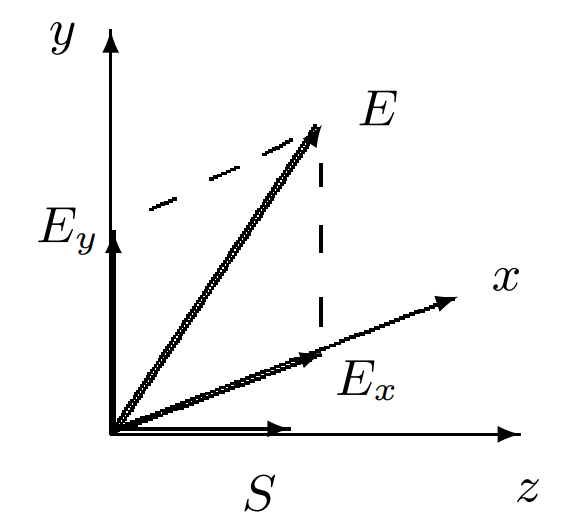
\includegraphics[width=\linewidth]{fig1}
	\caption{Представление световой волны в виде двух линейно поляризованных волн}
\end{wrapfigure}


При помощи специальных приспособлений (поляризаторов), о которых речь будет идти дальше, естественный свет может быть превращен в \textit{линейно поляризованный}. В линейно поляризованной световой волне пара векторов \textbf{E} и \textbf{H} не изменяет с течением времени своей ориентации.

Наиболее общим типом поляризации является эллиптическая поляризация. В эллиптически поляризованной световой волне конец вектора \textbf{E} (в данной точке пространства) описывает некоторый эллипс.

При теоретическом рассмотрении различных типов поляризации часто бывает удобно проектировать вектор \textbf{E} в некоторой точке пространства на два взаимно перпендикулярных направления (рис. 1). В том случае, когда исходная волна была поляризованной, $E_x$ и $E_y$ когерентны между собой и могут быть записаны в виде

\begin{equation}
\begin{gathered}
E_x = E_{x0} \cos(kz - \omega t), \\
E_y = E_{y0} \cos(kz - \omega t - \varphi),
\end{gathered}
\end{equation}

где амплитуды $E_{x0}$, $E_{y0}$, волновой вектор k,
частота $\omega$ и сдвиг фаз $\varphi$ не зависят от времени. Формулы (1) описывают монохроматический свет. Немонохроматический свет может быть представлен суммой выражений типа (1) с различными значениями частоты $\omega$.

В плоскости $z = z_0$ вектор \textbf{E} волны (1) вращается против часовой стрелки (при наблюдении навстречу волне), если 0 < $\varphi$ < $\pi$. В этом случае говорят о левой эллиптической поляризации волны. Если же $\pi$ < $\varphi$ < 2$\pi$, вращение вектора \textbf{E} происходит по часовой стрелке, и волна имеет правую эллиптическую поляризацию


\subsection*{Естественный и поляризованный свет}








\end{document}